% Chapter 4

\chapter{Challenges in Mining Event Related Content from Social Media} % Main chapter title

\label{challenges} % For referencing the chapter elsewhere, use \ref{Chapter1} 

\lhead{Chapter 4. \emph{Challenges in Mining Event Related Informative Content from Social Media}} % This is for the header on each page - perhaps a shortened title
\doublespacing
\setlength{\parindent}{1cm}
The characteristics of social media websites as discussed in Section \ref{char} of Chapter \ref{events}, makes the domain extremely unstructured and uncontrolled. This gives rise to different challenges in mining information from all types of social media platforms. Some of the major challenges applicable to the context of this dissertation are discussed below. The solutions to these challenges as proposed in this dissertation is also refered while explaining them. Social media posts from the datasets collected for the experiments in Chapter \ref{eiim} (Section \ref{eventreferencecollection}) are presented as examples while discussing the problems.

\section{Information Overload\label{informationoverload}}
A daily average of 58 million tweets is posted in Twitter\footnote{http://www.statisticbrain.com/twitter-statistics/}. On an average 60 million  photos are shared in Instagram daily\footnote{http://instagram.com/press/}. Facebook stores 300 petabytes  of data related to its users from all over the world\footnote{http://expandedramblings.com/index.php/by-the-numbers-17-amazing-facebook-stats/}. These are some compelling statistics that makes social media not only rich in volume of data, but also variety, and the velocity at which data is being generated. Due to the great pace at which data is produced in social media, the search engines and content filtering algorithms often face the problem of information overload \cite{hemp2009death}. They suffer from the dilemma of assessing the accuracy and quality of information content in the sources being produced over their freshness. Thus, collecting different types of references of events from social media, assessing their quality, resolving and extracting identity information of the events poses great challenges in such a situation. 

For example, 284 million monthly users of Twitter posting 500 million tweets per day produces a variety of content\footnote{http://about.twitter.com/company}. A significant proportion of it are related to different real-life events (e.g, football matches, conferences, music shows, etc). Majority of this content are personal updates (e.g.  \textit{Thanks for the memories Sochi! I've had the time of my life \#Sochi2014 \#sochiselfie http://t.co/DqkLEaAMpo}), pointless babbles (e.g. \textit{Ted Cruz is a dangerous man. Crazy and gaining support. Megalomaniac leaders are bad, mkay. \#CPAC \#politics \#joke}) and spams (e.g \textit{New post: Sochi Was For Suckers - Laugh Studios/ http://t.co/cWQJCBp3Ow \#lol \#funny \#rofl \#funnypic \#wtf.}). Personal views and conversations might be of interest to a specific group of people. However, they are meaningless and provides no information to the general audience. On the other hand there are tweets that presents newsworthy content, recent updates and real-time coverage of on-going events (e.g. \textit{In \#Sochi, the Dutch are dominating the overall Olympic medal count http://t.co/jMR1WUqEK4 (Reuters) http://t.co/dAfDhEgTGA}). These tweets provide event-specific informative content and are more useful for the users interested to know about the event. In this dissertation, we call them as event-specific informative tweets. One of the main problems due to information overload is to identify these tweets among millions of tweets being produced during the event. Table \ref{tweetsample} presents some examples of different types of tweets shared during real-life events.

Techniques are developed in this dissertation that overcomes this challenge. In Chapter \ref{eiim} (Section \ref{eventinfoquality}), a generic supervised classifier for Twitter is developed in order to identify event references in real-time that has greater chances of containing high quality information. This results in segregation of informative references from the non-informative ones, and identification of the informative references for further processing. The \textit{EventIdentityInfoRank} algorithm implemented in Chapter \ref{eiim} (Section \ref{eventidentityinforank}), processes the content in the filtered tweets and results in a ranked list of tweets that has high quality event-specific informative content. 

\begin{table}[htbp]
\centering
\caption{Examples of different event related tweets.}
\label{tweetsample}
     \begin{tabular}{|p{14cm}|} \hline
     Ted Cruz is a dangerous man. Crazy and gaining support. Megalomaniac leaders are bad, mkay. \#CPAC \#politics \#joke [\textit{\textbf{personal/uninformative}}] \small \textit{\textbf{Event: `CPAC 2014'}}\\ \hline
     Thanks for the memories Sochi! I've had the time of my life \#Sochi2014 \#sochiselfie http://t.co/DqkLEaAMpo. [\textit{\textbf{personal/uninformative}}] \small \textit{\textbf{Event: `Sochi Games'}} \\ \hline
     \#SXSW14 \#SXSW \#sxswinteractive \#CPAC2014 \#CPAC \#CPACPickupLines \#CPACPanels Be squared away \@ perky TOP TWEETED of http://t.co/h0igdOVNW0. [\textit{\textbf{spam/uninformative}}] \small \textit{\textbf{Event: `CPAC 2014'}}\\ \hline
In \#Sochi, the Dutch are dominating the overall Olympic medal count http://t.co/jMR1WUqEK4 (Reuters) http://t.co/dAfDhEgTGA. [\textit{\textbf{event-specific informative}}] \small \textit{\textbf{Event: `Sochi Games'}}\\ \hline
New post: Sochi Was For Suckers - Laugh Studios/ http://t.co/cWQJCBp3Ow \#lol \#funny \#rofl \#funnypic \#fail \#wtf. [\textit{\textbf{spam/uninformative}}] \small \textit{\textbf{Event: `Sochi Games'}}\\ \hline
It's \@tedcruz vs. \@SenJohnMcCain in a \#CPAC spat. What did they say? Find out on \#AC360 8p on \@CNN. [\textit{\textbf{event-specific informative}}] \small \textit{\textbf{Event: `CPAC 2014'}} \\ \hline
     \end{tabular}
\end{table}

\section{Veracity of Sources\label{veracity}}
Judging the accuracy of the information and detecting relevant, event-specific informative content from social media constitutes another challenging situation due to the malevolent practices of spam users. For trending topics, the search engines have started showing real-time feeds from social media websites in their search results. This has attracted spammers who post trending hashtags or keywords along with their spam content in order to attract people to their websites offering products or services \cite{benevenuto2010detecting}. For example, the tweet (\textit{RT @BFDealz: http://t.co/TSJAigrVJI WHEELS SUPER TREASURE HUNT SUPERIZED HARLEY DAVIDSON FAT BOY LONG CARD 2014 \#cpac2014 \#sxsw}) was posted during the parallel occurrence of CPAC 2014 (a political conference) and SXSW 2014, but has nothing to do with the events. Instead it leads to a deal related to Harley Davidson bike promoted using popular event related hashtags \#cpac2014 and \#sxsw. 

An alarming 355\% growth of spam in social media has been reported in 2013\footnote{http://www.likeable.com/blog/2013/11/10-surprising-social-media-statistics/}. Social media has also been instrumental in spreading misinformation and rumors. Spread of misinformation not only results in pandemonium among the users\footnote{http://www.theguardian.com/uk/interactive/2011/dec/07/london-riots-twitter}  but also result in extraction of completely wrong information about events. The users in the social media websites also develop nepotistic relationships in order to get higher scores in the ranking techniques with malicious intentions \cite{gayo2013nepotistic}. This also helps them to spread spam and other malicious content. Such behavior can also lead to cyber attacks.

Some examples of spam tweets in the collected dataset are shown in Table \ref{tweetsample}. Most of the existing techniques face problems in combating spam.  \textit{EventIdentityInfoGraph} (Section \ref{eventidentityinfograph}) is presented and explained in this dissertation that defines mutually reinforcing chains in Twitter for identifying the most event-specific informative references and filters out the spam tweets after ranking its nodes using \textit{EventIdentityInfoRank} (Section \ref{eventidentityinforank}). The algorithm can also identify users who are producing event-specific informative content and URLs (images, videos, news articles) that are extremely relevant to the event. 

\section{Multiple Data Sources with Variety of Content}
The APIs (Application Programming Interfaces) of the different social media websites returns data in different formats (JSON, XML) using different web standards (REST, HTTPS). Moreover, the information obtained from a social media website is dependent upon the type of content it produces. A video sharing website might return an entirely different set of information from a blogging website. Thus, integrating the data obtained from various social media platforms for the purpose of tracking and extraction of event related information is one of the many challenges.

Although, type and format of the data returned by the social media services vary, yet most of them have certain common meta-data associated with messages obtained in response to the API requests. These are hashtags, text units extracted from the messages/descriptions, the messages itself, the users posting them and the URLs that lead to external sources of information. Some of the websites where hashtags are not present, the associated tags can be used instead. Table \ref{socialmediametadata} shows the presence of these meta-data in the most popular social media platforms.

\begin{table}[h]
\caption{Presence of different meta-data in popular social media websites.}
\label{socialmediametadata}
\centering
\begin{tabular}{|c|c|c|c|c|c|}
\hline
\textbf{\begin{tabular}[c]{@{}c@{}}Social Media/\\ Website\end{tabular}} & \textbf{Hashtags} & \textbf{Users} & \textbf{Text Units} & \textbf{\begin{tabular}[c]{@{}c@{}}Messages/\\ Description\end{tabular}} & \textbf{URLs} \\ \hline
\textit{\textbf{Facebook}} & Yes & Yes & Yes & Yes & Yes \\ \hline
\textit{\textbf{LinkedIn}} & Yes & Yes & Yes & Yes & Yes \\ \hline
\textit{\textbf{Pinterest}} & Yes & Yes & Yes & Yes & Yes \\ \hline
\textit{\textbf{Instagram}} & Yes & Yes & Yes & Yes & Yes \\ \hline
\textit{\textbf{Twitter}} & Yes & Yes & Yes & Yes & Yes \\ \hline
\textit{\textbf{Flickr}} & Yes & Yes & Yes & Yes & Yes \\ \hline
\textit{\textbf{Google Plus}} & Yes & Yes & Yes & Yes & Yes \\ \hline
\textit{\textbf{YouTube}} & Yes & Yes & Yes & Yes & Yes \\ \hline
\end{tabular}
\end{table}  

The developed techniques that are explained in this dissertation rely only upon the above meta-data. This makes the techniques generic and useful for most of the social media channels.
 

\section{Informal Text}
Unlike sources of news media and edited documents on the web, the textual content of the social media references are highly colloquial and pose great difficulties in extracting information. One of the most important sources of information about events, prevalent in the domain of social media are the micro-blogging platforms. Micro blogs pose additional challenges due to their brevity, noisiness, idiosyncratic language, unusual structure and ambiguous representation of discourse \cite{bontcheva2013twitie}. Variation in language, less grammatical structure of sentences, unconventional uses of capitalization, frequent use of emoticons, and abbreviations have to be dealt by any system processing social media content. Moreover, various signals of communications embedded in the text in the form of hash-tags (eg.\#sochi), retweets (RT) and user mentions (@) should be understood by the system in order to extract the contextual information hidden in the text. Intentional misspellings sometimes demonstrate examples of intonation in written text \cite{prevost1996information}. For instance, expressions like, `this is so cooool', emphasizes stress on the emotions and conveys more information that should be captured. It has been shown that it is extremely challenging for the state-of-the-art information extraction algorithms to perform efficiently and give accurate results for micro-blogs \cite{derczynski2013microblog}. For example, named entity recognition methods typically show 85-90\% accuracy on longer texts, but 30-50\% on tweets \cite{ritter2011named}. Status messages in social networking websites, content in question answering websites, reviews, and discussions in blogs, and forums exhibit similar nature and present similar challenges to information extraction and text mining procedures.

In order to solve some of these problems additional resources are compiled in the dissertation. Some of these resources are list of slang words, list of acronyms and list of stop words commonly used in short social media text (refer Chapter \ref{eiim}). These resources are used to aid the natural language processing techniques, resulting in their better performance. Experiments were also performed using the state-of-the-art entity extraction service, AlchemyAPI\footnote{http://alchemyapi.com} (Chapter \ref{eval}). The final results obtained using the data processing pipeline developed in this dissertation gave better results than AlchemyAPI for short textual content in social media.



\section{Searching for Information in Long Tail}

\begin{figure}[htbp]
\centering
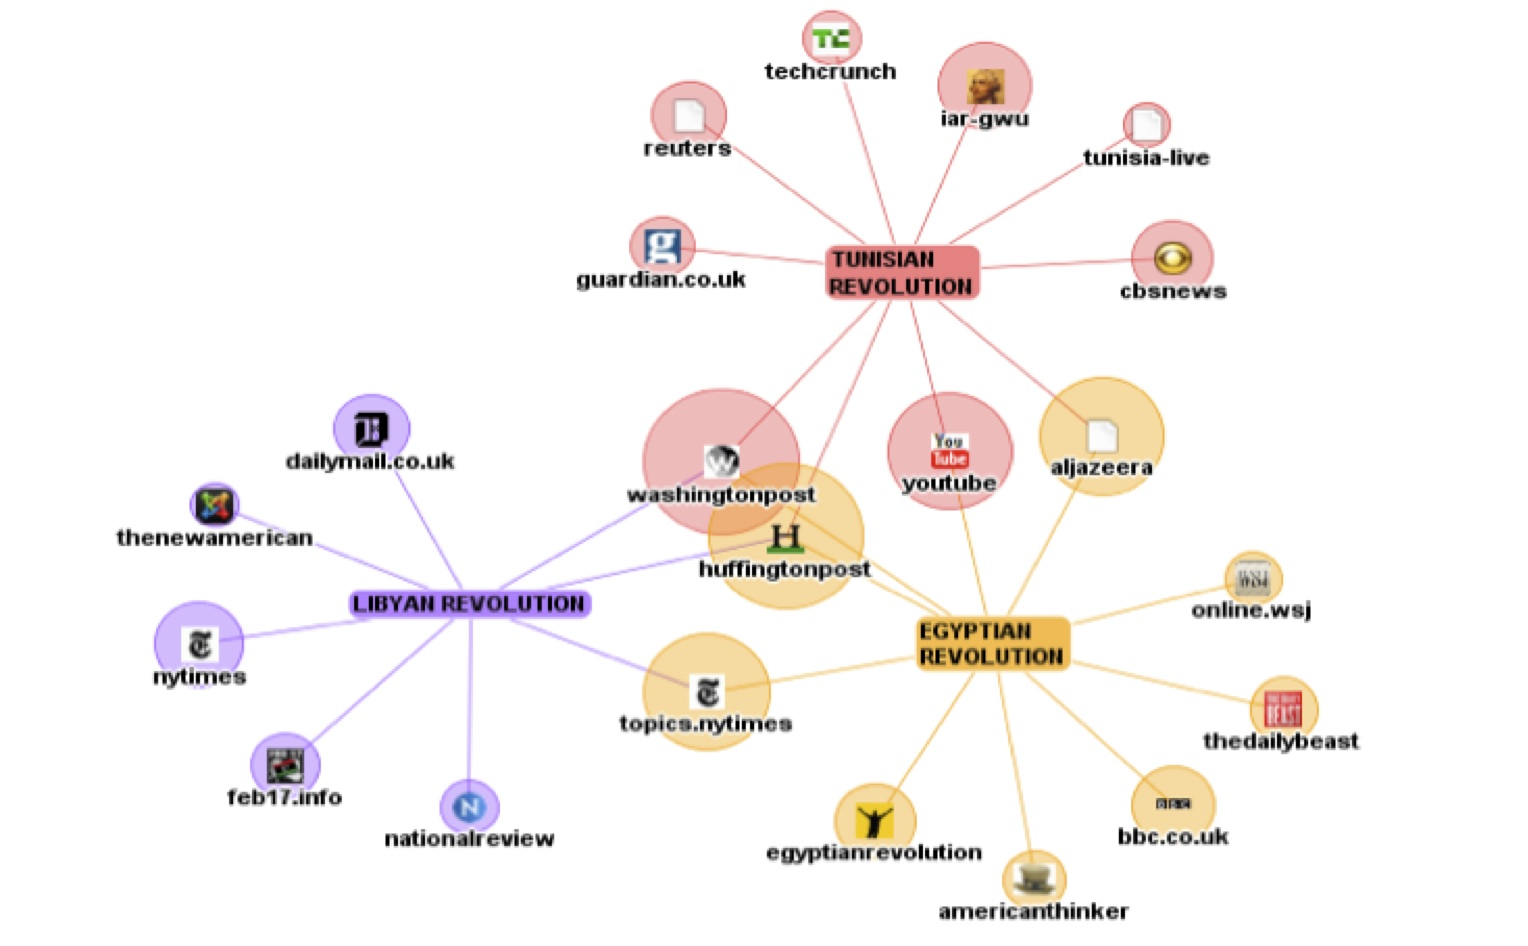
\includegraphics[height=3.5in,width=4.5in]{Figures/Chapter3Figures/touchgraph.jpg} 

\caption{Top 10 Google search results for ``Egyptian Revolution'', ``Libyan Revolution'', and ``Tunisian Revolution'', visualized using TouchGraph.}

\label{fg:touchgraph}

\end{figure}

\begin{figure}[htb]
\centering
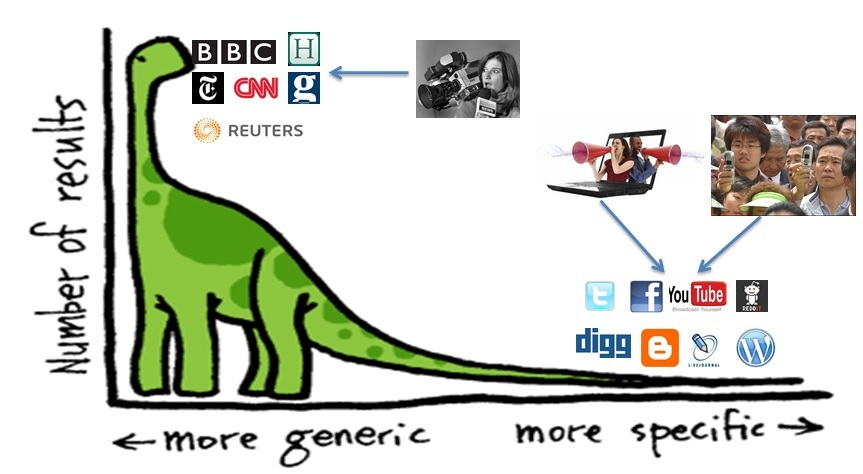
\includegraphics[height=3.3in,width=4.8in]{Figures/Chapter3Figures/LongTailVsShortHead.jpg} 

\caption{Short Head Vs Long Tail media sources.}

\label{fg:longvsshort}

\end{figure}


Due to the power law distribution of the Internet \cite{adamic2000power}, and the present search engine technology, the `Short Head' is generally dominated by the mainstream media websites. As illustrated in Figure ~\ref{fg:touchgraph} the top 10 search results for ``Egyptian Revolution", ``Libyan Revolution", and ``Tunisian Revolution" by Google, visualized using Touchgraph\footnote{http://touchgraph.com}, mostly retrieved mainstream media references. Consequently, the social media sites get buried in the Long Tail \cite{LOmariba} as shown in Figure ~\ref{fg:longvsshort}. However, references from the social media channels, act as hubs of relevant information about real-life events \cite{harb2011arab}. On the other hand, the mainstream media sources often gloss over the intricate details while covering a real-life event. They are often biased, regulated by the government, and may not portray the true picture of an event \cite{hamdy2012framing}. While, social media references often contain unbiased, uninhibited, and unedited opinions from people. Political blogs have been accepted as more credible sources of information over mainstream media references by the weblog users \cite{johnson2004wag}. Thus the references, which are obtained from social media could potentially provide a rather `closer'  or an ``on-ground" view of the events with novel information. The ``on-ground'" information gleaned from the social media affords opportunities to study various online social phenomenon from methodological and theoretical perspectives including, social movements, crowdsourcing, citizen journalism, collective behavior, collective action \cite{agarwal2011finding,agarwal2012online,agarwal2012raising}, and more.

\begin{figure}[htbp]
\centering
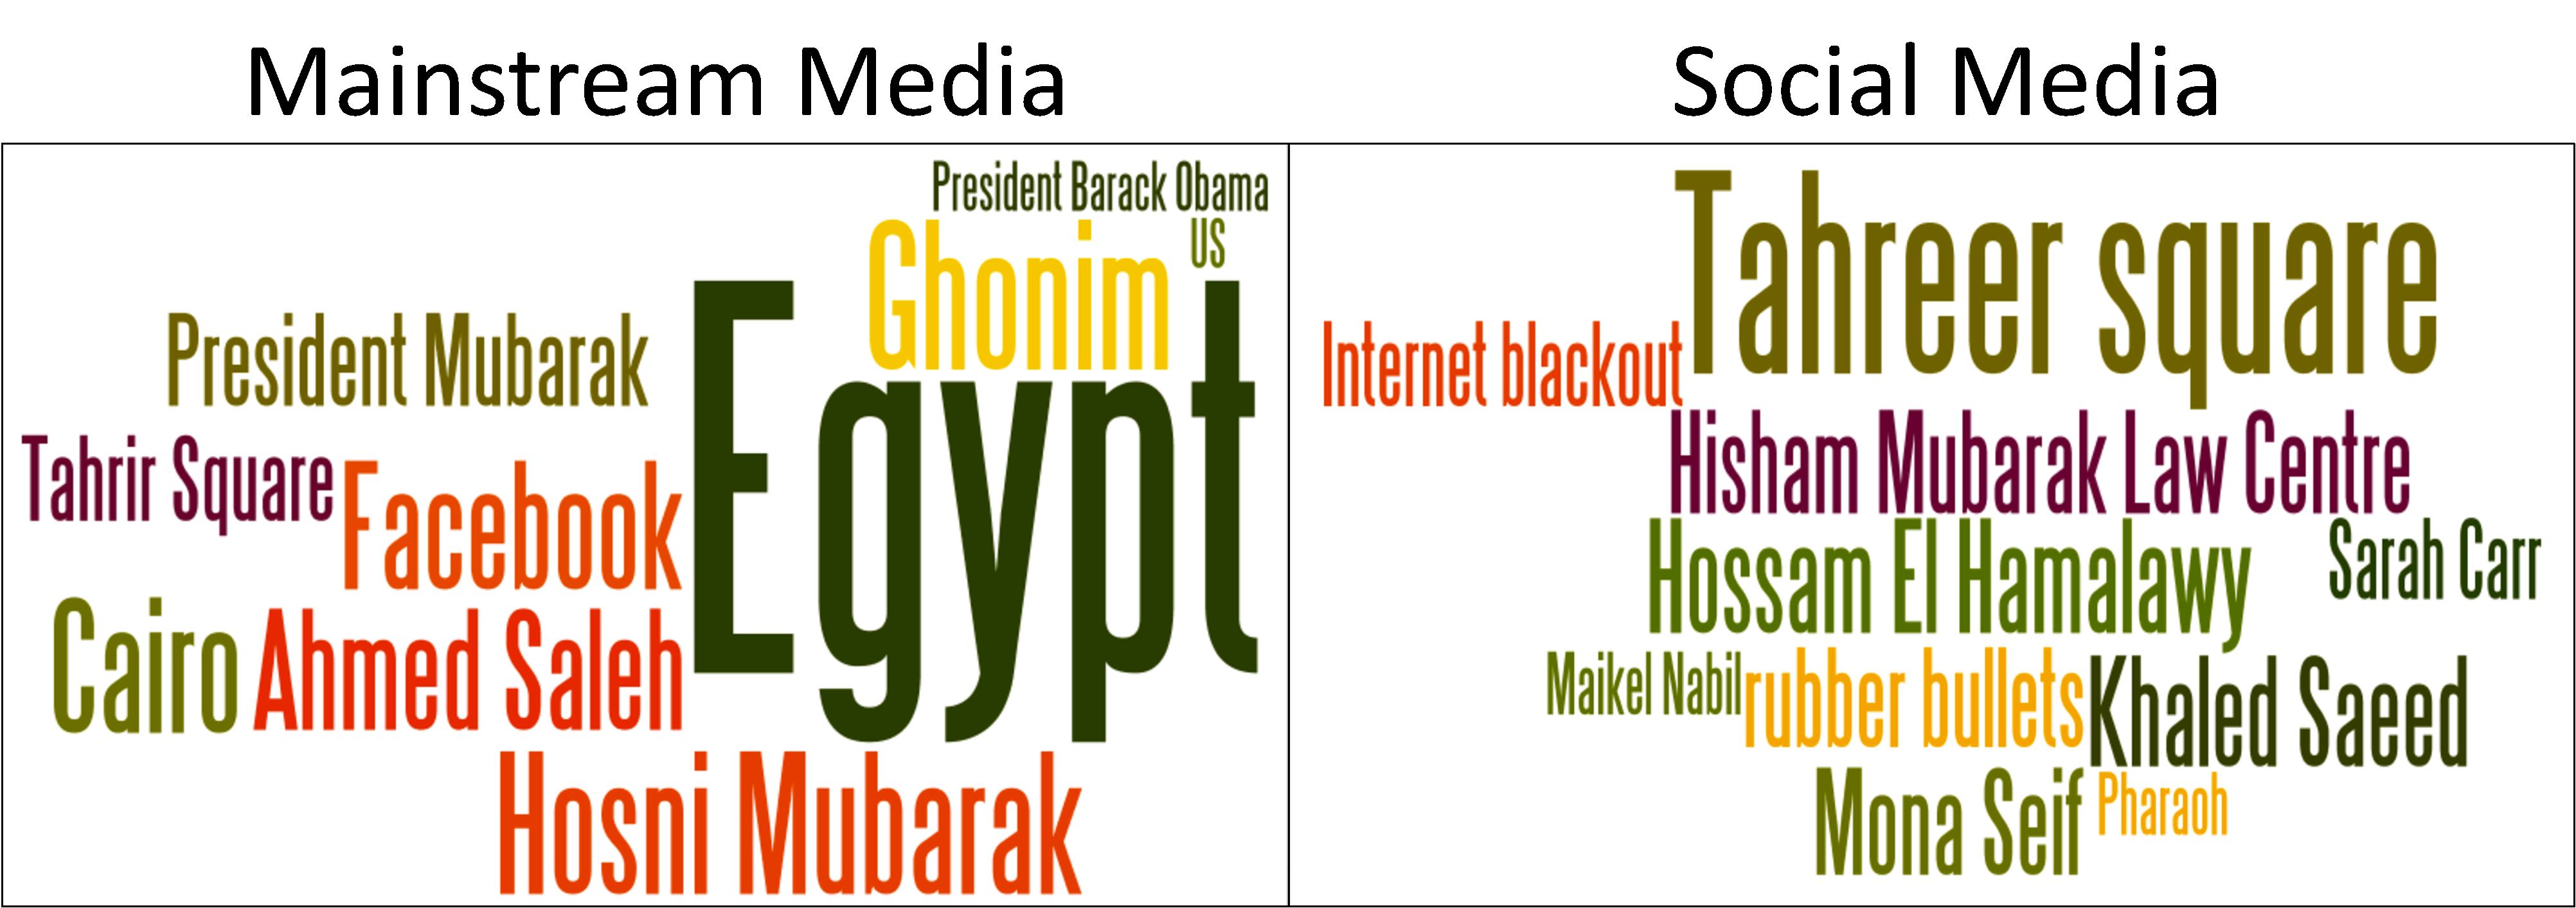
\includegraphics[height=2in,width=4.5in]{Figures/Chapter3Figures/comp.pdf}
\caption{Top 10 entities from mainstream media and blogs.}
\label{fg:comp}
\end{figure}

An initial analysis of the top 10 entities obtained from the top 10 search results related to ``Egyptian Revolution'' from two mainstream media channels (BBC and CNN), and from blogs during the time of the revolution is shown in Figure~\ref{fg:comp}. The top entities from the mainstream media channels are generic and are quiet obvious for the event. In contrast, the top entities from the blogs are very specific to the event. The activists like `Mona Seif', `Sarah Carr', `Maikel Nabil' and `Hosam El Hamalwy' were very closely involved, and were responsible for mobilizing the event. The entities like `Internet Blackout' and `Khaleed Saeed' were central to the event. Moreover, the presence of entities like `Facebook' and `Ghonim' (who was responsible for spreading the event in Facebook) among the top mainstream media entities also indicates the significance of social media in the event.

A person interested to know about an event in detail, may miss out the novel and specific information available in social media by relying on the top results from the popular search engines. It is a challenge for the current ranking schemes to retrieve the event-specific social media content from the long tail. Moreover, in the words of Chris Anderson \cite{anderson2008long}, \begin{itshape} ``With an estimated 15 million bloggers out there, the odds that a few will have something important and insightful to say are good and getting better.'' \end{itshape} This also motivated to look for techniques in this dissertation, that would help in identifying these otherwise buried sources providing highly specific information related to an event.

\section{Sparse Link Structure}
The casual nature of the users posting content in social media channels gives rise to the challenge of sparsity in link structures. Most often the users who posts content, do not provide links to the original source of information. Also, the behavior of linking to other similar content or building citation networks between information posted about the same topic is completely absent among the social media users. This creates an extremely sparse link structure between the user-generated posts. This further creates problems for the traditional and state-of-the-art searching techniques such as PageRank \cite{brin1998anatomy} that performs well in ranking web pages.

This dissertation, introduces and defines novel implicit relationships, intrinsic to content available in the social media channels for solving this issue, and ranks them showing better performances than some of the popular techniques.  


\section{Sampling Bias}
Most commonly used method for obtaining data samples from social media websites is by using their application programming interfaces (APIs). Given the humungous amounts of data produced in real-time, the APIs cannot provide all the data to every single API requests. The requests are often made through a query interface by passing certain query parameters to the APIs. The amount of data returned against the queries may vary. This depends upon the popularity of the content related to the query. For example, in Twitter, studies have estimated that by using Twitter's Streaming API users can expect to receive anywhere from 1\% of the tweets to over 40\% of tweets in near real-time\footnote{https://www.brightplanet.com/2013/06/twitter-firehose-vs-twitter-api-whats-the-difference-and-why-should-you-care/}. The only way to get access to all the tweets is to buy the firehose service, which is seldom done for academic purposes. Other real-time social media publishing services mostly follow the same model. Therefore, this might lead to biasness in the samples collected for studying event related phenomenon and for tracking all the important event related information being produced in real-time.


\section{Lack of Evaluation Datasets}
There is a lack of ground truth evaluation data for most of the social media text mining tasks. In traditional data mining research, there is often two types of datasets. One of them is known as training dataset and the other is known as test dataset. The models are trained or developed using the training datasets and are evaluated on test datasets. Thus, the test datasets act as the ground truth. The test dataset for various text mining tasks is mostly not available for social media. It is often the duty of the researchers to create new test datasets in order to solve a specific task in social media. Sometimes this data might not be a benchmark dataset due to various unwanted noise and human error or perception in annotating the data. This might lead to wrong assumptions and false results.

Popularly used validation techniques that are widely accepted by the research community for circumventing the evaluation challenges are used in this dissertation. Both automated as well as manual methods of evaluation, are considered according to the scenario. Independent annotators are used for all the annotation tasks. They are properly educated about the tasks and the events. Please refer (Chapter \ref{eval}) for more details.
